\documentclass[10pt, english, pra,aps,twocolumn,floatfix,superscriptaddress]{revtex4-2}

\usepackage[utf8]{inputenc}
\usepackage{graphicx}
\usepackage{dcolumn}
\usepackage{bm}
\usepackage{float}

\usepackage[pdfstartview={FitH},bookmarks=false]
 {hyperref}

\usepackage{dsfont}
\usepackage{amsmath,tikz}
\usetikzlibrary{matrix}
\usepackage{amsmath}
\usepackage{braket}
\usepackage{caption}
\usepackage[left=1.5cm,right=1.5cm]{geometry}
\usepackage{graphicx}
\usepackage{dcolumn}
\usepackage{bm}

\begin{document}

\title{Searching for Cherenkov in the Sky}
\author{Reyhaneh Aghaei Saem}
\email{reyhaneh.aghaei@physics.sharif.edu}
 \affiliation{Department of Physics, Sharif University of Technology}
\author{Zahra Farahmand}
 \email{zahra.farahmand@physics.sharif.edu}
\affiliation{Department of Physics, Sharif University of Technology}
\author{Bahar Nikbakht}
 \email{bahar.nikbakht@physics.sharif.edu}
\affiliation{Department of Physics, Sharif University of Technology}
% \author{Ali Akbar Abolhasani}
%  \email{abolhasani@ipm.ir}
% \affiliation{Department of Physics, Sharif University of Technology}
% \author{Sadegh Raeisi}
%  \email{sraeisi@sharif.edu}
% \affiliation{Department of Physics, Sharif University of Technology}



\begin{abstract}
In a recent paper, AA. Abolhasani and S. Jazayeri have claimed that the production of additional relativistic particles coupled to the inflation can cause imprints like Cherenkov effect on the temperature anisotropies of CMB. In this article we have tried to find these traces and used 45000 simulated data sets and Convolution Neural Network (CNN) in order to find a proper network to look for them in Planck 2018 data release.Finally, we found that if these traces exist, then their excess on CMB data could not be significantly greater than the background noise.
\end{abstract}

\maketitle
    
\section{Introduction}
Today, Cosmology has made great strides thanks to accurate observational data among which is the observation of Cosmic Microwave Background (CMB), which is in perfect agreement with the widely accepted inflationary $\Lambda$CDM model\cite{2018planck}. In this model, considered as the standard model of cosmology, it is assumed that the universe, in the early stages of its evolution, has undergone an exponential expansion phase called inflation\cite{guth,Starobinsky:1980te,Linde:1981mu}.

In the inflationary scenarios, primordial density and gravity-wave fluctuations are originated from the quantum fluctuations which are stretched and cross the horizon and frozen there, and eventually, considering as the seeds for Large Scale Structures(LSS)\cite{Bartolo_2004}.These perturbations at the surface of the last scattering are observable as the temperature anisotropies of the CMB.

Planck satellite has confirmed that the initial seeds of structure, or equivalently CMB temperature map, must have been close to Gaussian and isotropic\cite{Akrami_2020,isotropy}. This is almost the same as what we expect from single-field inflationary models\cite{single-field}, and puts important constrains on a notable fraction of inflationary models in which detectable non-Gaussianities is expected, i.e. multifield inflation\cite{NG-multifield,Planck_inflation}.

On the other hand, some models motivated by high energy physics suggest detectable signatures of primordial non-Gaussianities with a unique shape, hereinafter called "Anomalies"\cite{Anomaly}. In recent years, various proposals for CMB anomalies and finding them have been suggested, among which we can mention Cosmic strings\cite{CS,CS2}. As we have already mentioned, since non-Gaussianity directly probes the dynamics in the early universe, a detection would present a monumental discovery in cosmology, providing clues about physics at energy scales as high as the GUT scale\cite{PNG,meerburg2019primordial}.

In this article, we intend to look for one of these anomalies suggested by A.A Abolhasani and S. Jazayeri\cite{AAA}. In this model, it is claimed that the production of localized relativistic sources due to the decay of heavier particles which are the results of resonance mechanism, can lead to an inflationary cherenkov effect. This effect appears in the form of specific patterns on the temperature anisotropies of the CMB, and by detecting them we will be able to obtain the speed of sound for scalar perturbations.

Each of the relativistic particles can produce one of these Cherenkov patterns on the temperature anisotropies of the CMB. Now if the number of these particles per Hubble time per Hubble patch is such that the trace of each of them can be distinguished from the others, for a particle that moves along the trajectory $x_A = \hat{q}\eta$ , the scalar emission $\zeta(\boldsymbol{x}, 0)$ for $\boldsymbol{x}$ well separated from the creation point, is given by,

\begin{equation}
\label{eq:zeta}
\zeta(\boldsymbol{x}, 0)=g_{\mathrm{eff}} \frac{2 A_{s}^{1 / 2} c_{s}^{1 / 2}}{(2 \pi) q_{n}} \frac{1}{\sqrt{(\boldsymbol{x} \cdot \hat{q})^{2}-\left(1-c_{s}^{2}\right) r^{2}}}.
\end{equation}

Where $A_s$ is the amplitude of the primordial scalar fluctuations, and $q_{n}$ is the comoving momentum of the particle, $c_s$ is the speed of sound and $g_{\mathrm{eff}}$ is the dimensionless coupling between the canonically normalized scalar field and the relativistic particle.It is easy to see that the equation \ref{eq:zeta} diverges for $(\boldsymbol{x} \cdot \hat{q})=\sqrt{(1-c_{s}^{2}} r$, which is the familiar equation of Mach-Cones.

According to the above description, the temperature fluctuations can be estimated as,
\begin{equation}
\label{theta}
    \Theta(\hat{\mathrm{n}}) \propto \zeta\left(r_{L} \hat{\mathrm{n}}\right),
\end{equation}
 where $r_L$ denotes the radial coordinate to the last scattering surface.

In this article, we have used machine learning methods to search for these traces on CMB. We first found a suitable method for generating the data and examined the extent of each of the parameters. Then we tried to find a suitable network that could detect these traces well, and finally we tested our model on CMB.

\section{Method}
We have used Convolutional Neural Network (CNN), to look for traces of inflationary Cherenkov. For this purpose, we first used CMB simulated maps and maps containing Cherenkov using the equation \ref{eq:zeta} in order to train our model and test the capability of it.Then we went to the real CMB and looked for the above traces.It is also worth mentioning that we have used the healpy library to perform all the above steps, in which spherical maps are divided into twelve patches, each patch being a square of NSIDE$\times$NSIDE pixels\cite{Gorski_2005}.In fact, NSIDE gives the total number of pixels, and the higher it is, the higher the resolution of the map.

In the following, we will first give a brief overview of the method we have used for simulations, then describe briefly the model we have trained.
\subsection{Data Sets}
We have gone the same procedure as\cite{Vafaei_Sadr_2017}, and used maps which were the superposition of two maps to learn the machine.The first maps were CMB simulations based on cosmological parameters from Planck 2018 data release\cite{2018planck}, and we have normalized them in a way that their standard deviation is one and the average of the data is zero. And the second maps were maps containing Cherenkov traces.

To simulate Cherenkov traces, we first use equations \ref{eq:zeta} and \ref{theta} to write the temperature anisotropies for each point as follows:

\begin{equation}
    \Theta(\hat{\mathrm{n}}) = \frac{1}{\beta} \times \frac{1}{\sqrt{(\boldsymbol{x} \cdot \hat{q})^{2}-\left(1-c_{s}^{2}\right) r^{2}}}.
\end{equation}
 Where $\beta^{-1}$ is a coefficient that contains all the constants of the above equations and in a way indicates the intensity of these Cherenkov traces.
 
 We know that Cherenkov traces appear in excess on CMB. On the other hand, we know that if we overestimate the intensity of these traces, the simulated data will be non-Gaussian, which is in contradiction with what is seen in real CMB. Also, underestimating the intensity of these traces will cause our machine to lose the ability to clean features from noise. Since the excess, seen on the CMB are very small, it is ideal for us to reduce the $\beta^{-1}$ value as much as the predictive power of our machine allows.
 
 On the other hand, the only parameter that is present in the physics of the problem with the length dimension is $r_L$. Therefore, we fix this parameter arbitrary and adjust the other parameters according to it. Here we got $r_L = 100$.
 
 Another parameter we need to determine is the number of relativistic particles that have the potential to intersect with the last scattering surface and create Cherenkov traces. As mentioned earlier, the number of these particles can not exceed a certain limit, because not only with a large number of particles the ability to follow them would lost but also, the Gaussianity we expect from the data would be destroyed. We call the number of particles n. We have also assumed that the particles are at the distance of $(-1.5\sqrt{3}\:r_L,+1.5\sqrt{3}\:r_L)$ at the recombination, and we also consider their direction to be random. It is important to note that not all n-particles we consider necessarily cross the last scattering surface.
 
 Final problem was that the above equation was too large for some values close to the boundary, while we know that CMB temperature anisotropies are in a certain range. To avoid this problem, we set a temperature limit, $\alpha$ and set all temperatures above $\alpha$ on the Cherenkov traces equal to $\alpha$. Thus, $\alpha$ is another parameter that must be carefully determined.
 
 For this purpose, we note that the larger the $\alpha$, the narrower and more explicit the boundaries we see Chernkov traces, and vice versa.
 
 In fact, $\alpha$ and $\beta$ parameters must be set simultaneously. And by changing these parameters, different traces of Cherenkovs can be achieved. Since we do not know the exact shape of these traces on the CMB, we have trained different values of these parameters,in a range expected from CMB. This is still a matter of debate, though.An example of Cherenkov's simulations can be seen in FIG \ref{fig:cherenkov}.
 
   \begin{figure}
     \centering
     \includegraphics[width=0.45\textwidth]{Cherenkov.jpg}
     \caption{An example of a simulated map of Cherenkov traces for $\alpha = 0.4$ and $\beta = 0.2$ for an ensemble of 6 particles, with NSIDE=2048.}
     \label{fig:cherenkov}
 \end{figure}
 
 
 As can be seen in FIG\ref{fig:cherenkov}, Cherenkov traces are not just a narrow line consisting of a set of points. Rather, they have a spatial scope and non-zero values within the Cherenkov boundaries. The specific shape of these traces and their specific temperature tolerances make us not worry about issues such as "look-elsewhere effect" that have already been raised for other presumed anomalies in CMB\cite{Anomaly,Moss_2011}.
 
 Then we were able to generate the right data for our neural network by overlapping CMB simulations and Chernkov simulations. In this way, we considered the maps containing CMB and traces as input and single traces as the desired data that must be learnt.
 
 But the problem was that considering NSIDE=2048 maps, which is the same as CMB in Planck data release, was very time consuming and inefficient. For this reason, we considered a flying window, using CCGPack\footnote{https://github.com/vafaei-ar/ccgpack}, that randomly moves through the various CMB patches that are assumed in the Healpix structure, separating parts of these maps and giving them to the machine as inputs.An example of the final structure of the data sets is provided in FIG \ref{fig:data}. We have called the side of these flying windows WSIDE, meaning that window possess WSIDE$\times$WSIDE pixels.
 
\begin{figure}
    \centering
    \includegraphics[width=0.45\textwidth]{sample_data.png}
    \caption{An example of the data sets we have used to learn our machine, with $\alpha = 0.5$,$\beta=0.2$ and NSIDE = 256}
    \label{fig:data}
\end{figure}

\subsection{Convolutional Neural Network Analysis}
In order to search for these traces, we tried to train our network using CNN methods so that it could find Chernokov traces in every window.

With some trial and error, we found that the proper structure for the network should be such that the number of channels first increases and then decreases and finally reaches one. We also used batch normalization at each stage, and found that filters with size 3$\times$3 are more appropriate, we have also used Mean Squared Error(MSE) for evaluating our model.

 We then tried to set the $\alpha$ and $\beta$ parameters so that the Cherenkov traces fade as much as our network can still detect it well. We finally reached $\alpha = 0.5$ and $\beta = 0.35$, and generate 45000 data sets with these parameter for the final run.
 
 We also used maps with NSIDE=256 to generate the data and fixed WSIDE=128. This will eventually lead to higher predictive power for maps with NSIDE=2048. Because when the total number of pixels increases, by keeping the number of pixels we have in the windows constant, the windows probe smaller areas of the whole map and seem to zoom in on the maps. This helps the network to separate Chernokov traces from noise better. Besides, it would help us with computational run time.
 
 Finally, to find other suitable parameters include learning rate, batch size and optimizer, we used the grid search and found that for Adam optimizer, batch size=128 and Learning rate = 0.001, the network is optimized. A predicted window can be seen in FIG \ref{fig:W_predict}.
 
  \begin{figure}
    \centering
    \includegraphics[width=0.45\textwidth]{sample_predict.png}
    \caption{An example of a predicted window the parameters of the traces are as follows: $\alpha=0.5$,$\beta=0.35$ and NSIDE = 256}
    \label{fig:W_predict}
\end{figure}
 
 In the next step, to predict complete maps, including simulated CMBs and Cherenkov traces, we first cut them into windows with WSIDE=128 pieces and gave them to the network. We then sewed the pieces together to get a complete map of what was predicted.FIG \ref{fig:map_predict} shows a predicted map.
 
 \begin{figure}
    \centering
    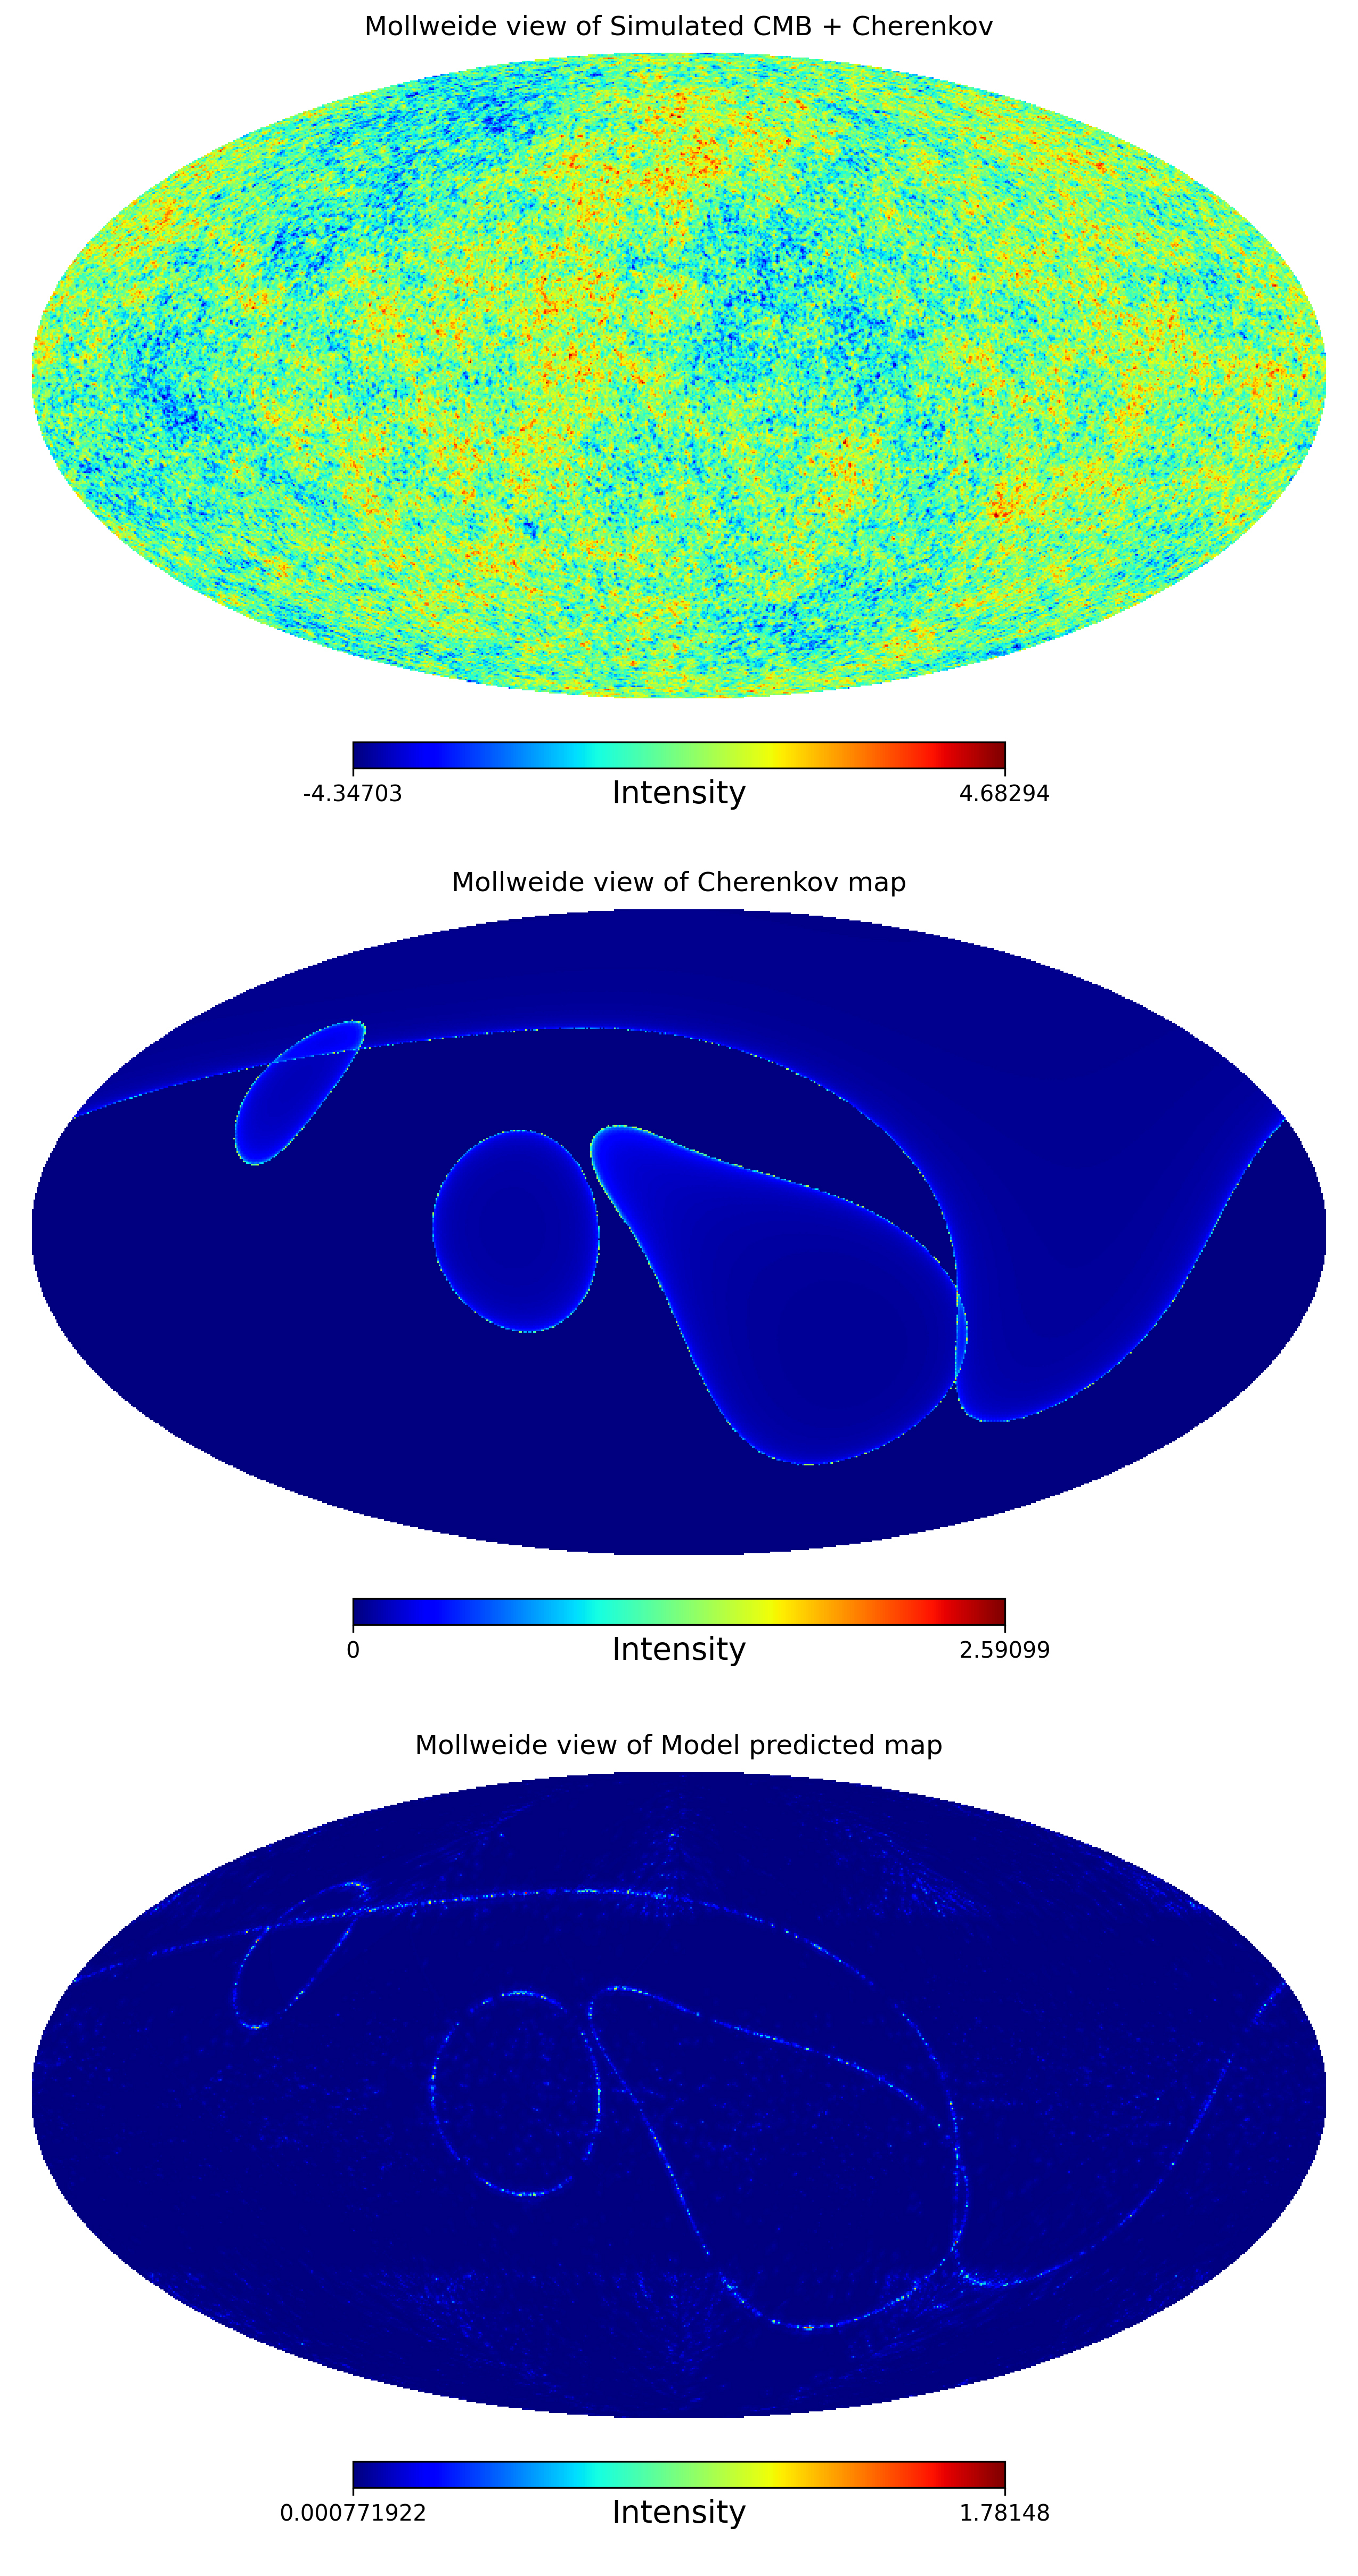
\includegraphics[width=0.43\textwidth]{mollview_map_total.jpg}
    \caption{A predicted map with $\alpha=0.5$,$\beta=0.35$ and NSIDE = 256}
    \label{fig:map_predict}
\end{figure}
 
\section{Results}
Now that we have our neural network ready, we can move on to the real CMB. We know that there are four different ways to clear CMB data: SMICA, NILC, SEVEM, and Commander\cite{collaboration2018planck}. The only difference between these maps is the way the data is cleaned. It should be noted that we need to discard all data that has been extrapolated into CMB data. For this reason, we only use maps whose masks have been published along with the data.Because of this, only two maps, SMICA and NILC, remain.

We bring the results for SMICA and NILC maps in FIG \ref{fig:CMB}.The initial results we get from these data are empty. However, the lack of these traces does not say anything about their impossibility. This just makes it difficult for us to keep going. We must continue to optimize our model and try to find parameters that put proper constrains on the intensity of these traces. It is also possible that current data are not accurate enough to detect these traces, and by development of the technology and enhancement of instruments we may be able to detect them better. In the future, we intend to examine the above claims carefully.

\section{Conclusion and Further Discussion}
In this paper, we investigate the possibility of observing inflationary Cherenkov traces in temperature anisotropies of CMB. For this purpose, we first found a suitable method for generating model-based data, then using this data and using CNN methods, we found a suitable structure for the network, and finally using the model we obtained to look for these traces on CMB. 

The initial result of our search for these traces in CMB was that the excess of them, if any, is less than $2\sigma$ of CMB data. Of course, the above statement is not an exact one, and we intend to use more precise constraints to determine the visibility of these traces by determining the parameters more precisely in the near future.

We aim to use three-layer maps instead of two-layer simulated maps, and include instrumental noise in the third layer, and for this purpose, we can use the noise which is common for telescopes.

 Then, in order to be more careful in predicting CMB maps and also to avoid edge effects, we are going to predict these maps several times. In a way that we first give the map to the network, then rotate it a bit, predicte it again, and rotate it in the opposite direction. And after repeating this process several times, we can finally average all predictions.

We also plan to use DeepSphere (Spherical CNN) instead of CNN to improve our model and see how efficient this method can be. The use of this method in analyzing CMB data has become very popular in recent articles of cosmological data analysis, and it seems that this method has been more effective for analyzing CMB so far\cite{DeepSphere}.

\section{Acknowledgement}
The above article has been prepared only as the final term paper of the Machine Learning Course instructed by Sadegh Raeisi. And this project is progressing with the contribution of Ali Alian, Reyhaneh Aghaei Saem, Zahra Farahmand and Bahar Nikbakht under supervision of Ali Akbar Abolhasani. We also thank Alireza Vafaee Sadr for helping to develop the main idea of this project.

 \begin{figure}
    \centering
    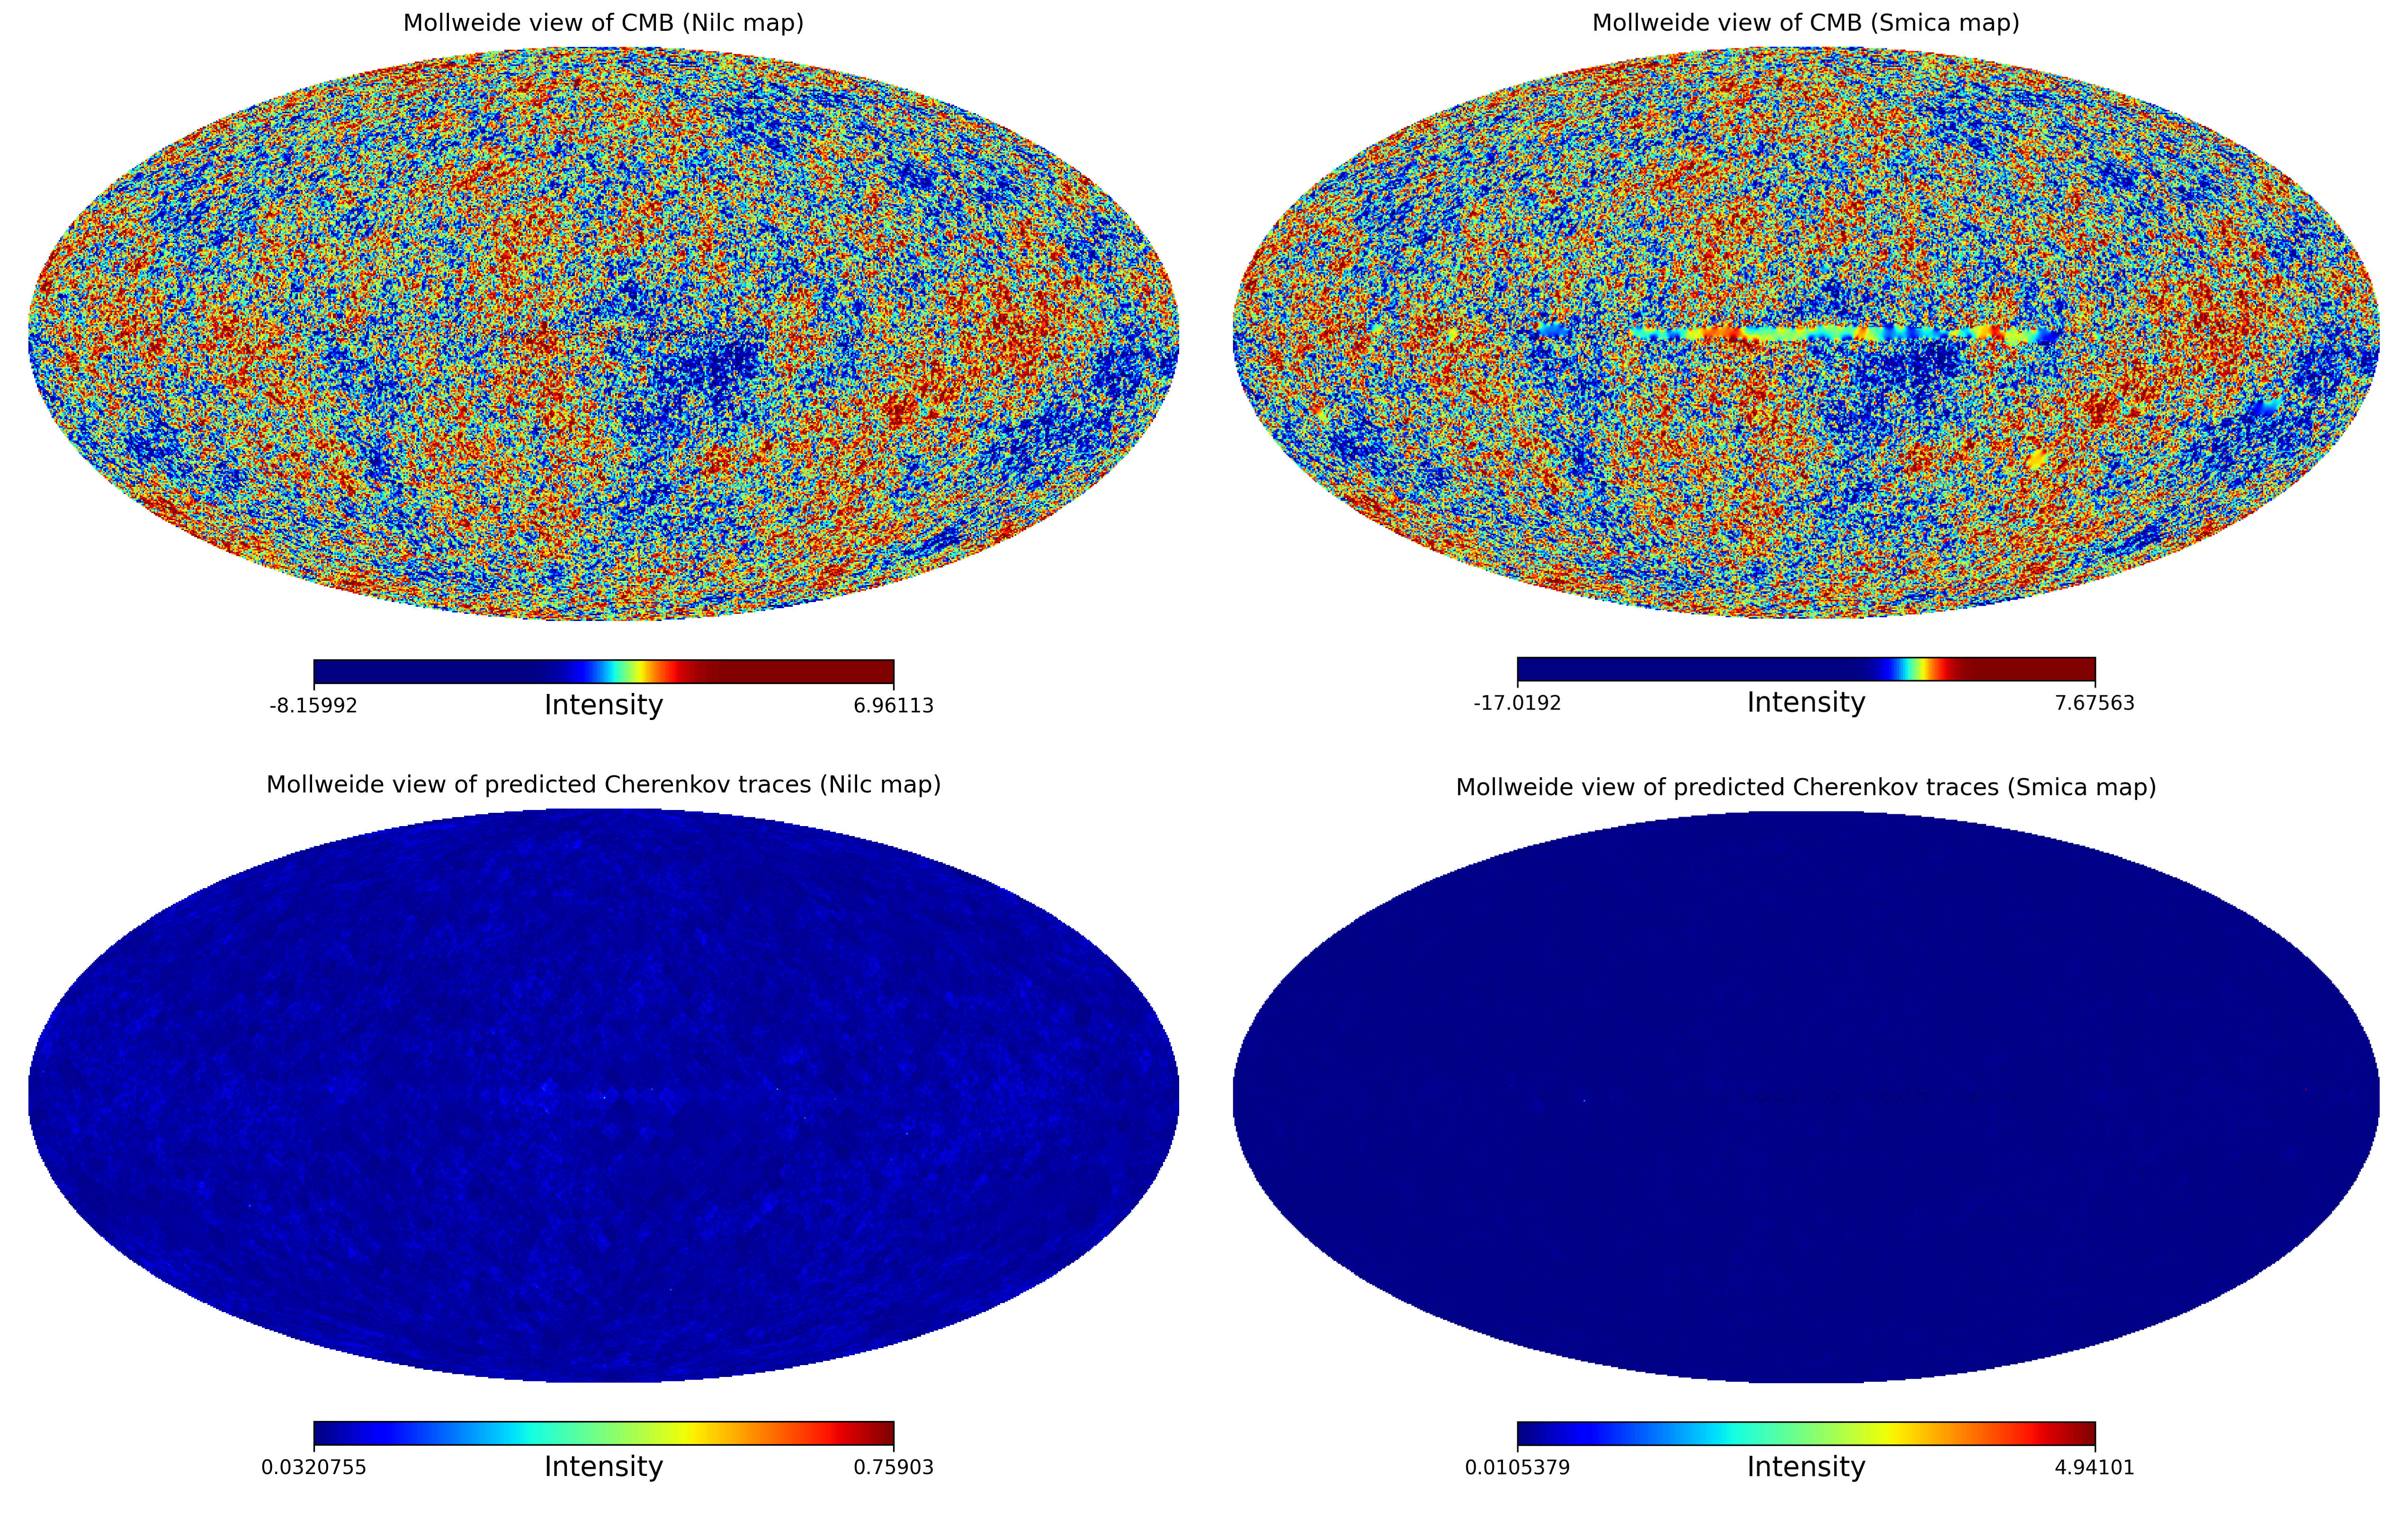
\includegraphics[width=0.9\textwidth]{CMB_maps.jpg}
    \caption{Predicted CMB maps:Nilc map(left) and SMICA(right)}
    \label{fig:CMB}
\end{figure}
\nocite{*}
\newpage
\bibliography{references}

\end{document}

